\section{Frontend (UIS, SV, Navigation)}
\label{sec:arch:frontend}
In diesem Projekt werden insgesamt drei auf Angular basierende Frontend-Applikationen erstellt. 
Diese sind grundsätzlich nach der Standardarchitektur von Angular aufgebaut. 
Deswegen werden zu Beginn des nachfolgendem Textes die Grundbausteine einer Angular-Applikation erklärt.

\subsection{Grundarchitektur von Angular}
Eine Angular-Applikation besteht grundlegend aus vier Bausteinen: das NgModule, Komponenten, Services und Interfaces.

\begin{figure}[!htb]
	\centering
	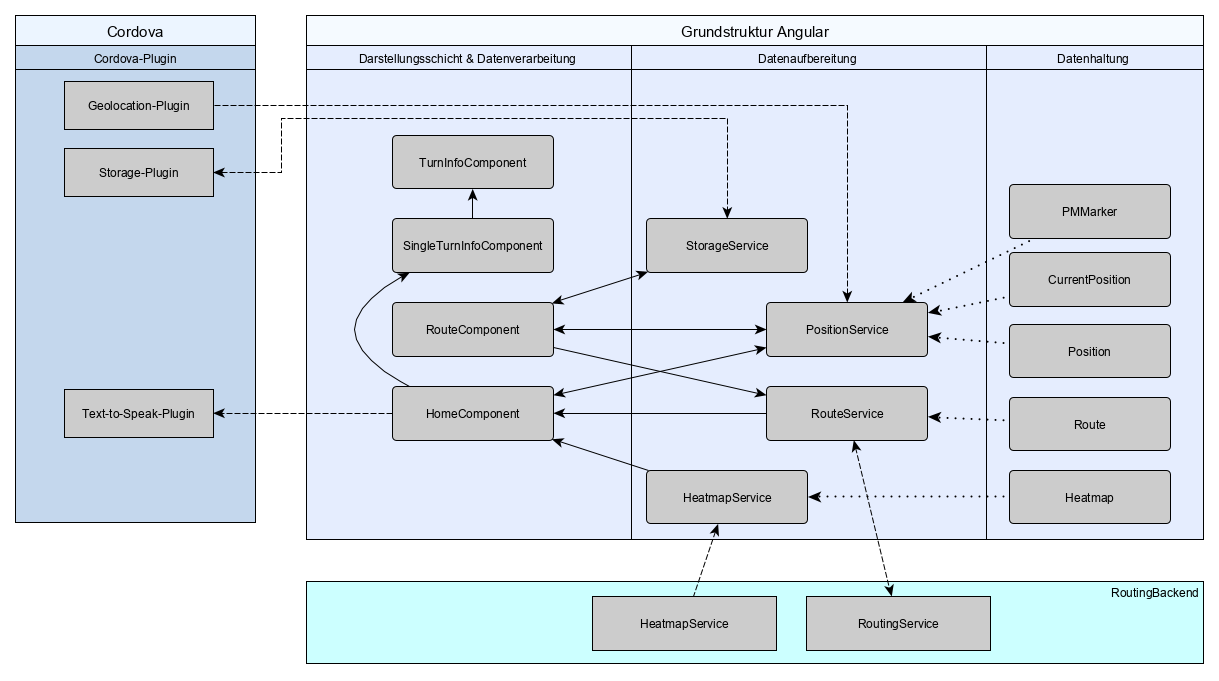
\includegraphics[width=\textwidth]{ressourcen/Architektur-Navigation}
	\caption{Überblick über die Bestandteile der Angular-Architektur}
	\label{fig:ArchtekturFrontend}
\end{figure}

\textbf{NgModule:}

Module deklarieren die für die Anwendung relevanten Komponenten, Funktionen und Workflows.
In diesen Dateien werden alle relevanten externen und internen Funktionalitäten, in Form von Services, Komponenten oder anderen Typen, integriert. 
Außerdem kann es andere NgModule integrieren, um deren Funktionalität zu übernehmen. 
Dies geschieht beispielsweise beim Integrieren externer Module, wie die Karte von Leaflet \cite{leaflet}.
Bei Leaflet handelt es sich um eine Bibliothek zum Darstellen von Karten in Apps oder auf Webseiten \cite{leaflet}. 
In jedem Angular Projekt gibt es dementsprechend immer mindestens ein Root-Module, welches mindestens die Hauptfunktionalität und die Startkomponenten integriert. 
Dies ist standardmäßig das AppModule mit der Integration der AppComponent.


\textbf{Komponenten}

Komponenten sind die verschiedenen Darstellungsbausteine, die in der Applikation angezeigt werden. 
Jeder dieser Komponenten besteht aus einer Html-Datei, die die Visualisierung auf einer Seite, auf Basis des Document Object Models (DOM), übernimmt. 
Diese besitzt ein dazugehöriges Stylesheet. 
In der Navigations- und in der UIS-Applikation wurde dafür die Stylesheet-Sprache Sass benutzt mit der Scss-Syntax, welche eine größere Funktionalität besitzt, als Cascading Style Sheets (Css). 
In der Sensorknotenverwaltungsapplikation werden Cascading Style Sheets benutzt. 
Zusammen ergeben die beiden Dateien das Template der Komponente. 
Jeder dieser Komponenten besitzt zudem eine TypeScript-Datei, die die Datenbereitstellung für die Html-Datei steuert. 
Dies wird durch das Databinding von Angular übernommen. 
Durch dieser Funktionalität können jede Art von Variablen und Funktionen an die html-Datei gegeben werden, die dort angezeigt oder für Funktionalitäten genutzt werden können.


\textbf{Services:}

In den Services werden logische Funktionen sowie die Bereitstellung von globalen oder externen Daten geregelt. 
Diese sind nach ihrer Funktion getrennt. 
Bei der Datenbereitstellung werden diese in die Klassen hineingegeben, die zuvor von der Klasse abgefragt wurden. 
Dies wird beispielsweise durch Observables umgesetzt. 
Dabei wird von der Klasse eine Variable abonniert, die bei einer Veränderung an alle Abonnenten weitergegeben werden. 
Eine weitere Funktion, die Services ist das Ansprechen und Abfragen von externen Schnittstellen.  


\textbf{Interfaces}

Interfaces geben die Grundstruktur von Datenobjekten vor und besitzen statische Funktionen. 
Durch diesen Datentypen werden in den einzelnen Projekten Objekte strukturiert, die in mehreren Funktionen vorkommen und ein genaue Struktur benötigen. 
Der größte Vorteil dieses Vorgehens besteht in der Warnfunktion von den IDEs. 
Diese zeigen bei einer falschen Nutzung von Variablen den Fehler auf, sodass eine falsche Nutzung von diesen Variablen nicht möglich ist. 
Beispielsweise werden im UIS-Frontend die Sensoren oder bei der Navigationsapplikation die Position damit strukturiert.


\textbf{Ebenen}

Die Grundstruktur der Frontend-Architektur unterteilt sich in vier Kategorien, wie auf \ref{fig:ArchtekturFrontend} ersichtlich ist. Die Darstellungsschicht, die Datenkomponenten, die Datenverarbeitung und die Datenhaltung. 
Diese Kategorien haben verschiedene Aufgaben, die sie in der späteren Applikation abbilden. 
Die Darstellungsschicht ist für die Visualisierung der Applikation und beinhaltet die html-Datei sowie die css-Datei der Komponenten. 
Diese bekommen ihre Daten von der Ebene der Datenkomponente. 
Zudem beinhaltet sie die ts-Dateien der Komponenten und Regeln den Event- und Variablen-Austausch mit der Darstellungsschicht. 
Außerdem sind diese auch für die Kommunikation mit der Datenverarbeitung zuständig. 
Diese Ebene besteht aus den Service, die in Form von ts-Dateien vorliegen. 
Solche Services haben die Aufgabe logische Berechnungen, Datenaufbereitung und die Kommunikation mit externen Schnittstellen durchzuführen. 
Für die Datenhaltung sind Interfaces genutzt worden, welche die Struktur von Daten vorgeben. 

\subsection{Komponenten}
Im nachfolgenden werden die einzelnen Frontends mit ihren spezifischen Ausprägungen vorgestellt und erklärt. 

\subsubsection{Navigation}
Die Navigationsapplikation ist mit dem Ionic-Framework gebaut. 
Die Programmierung basiert dabei auf Angular, mit der die Webansicht generiert wird, die dann mit Cordova in eine Android-Applikation übersetzt wird.

\begin{figure}[!htb]
	\centering
	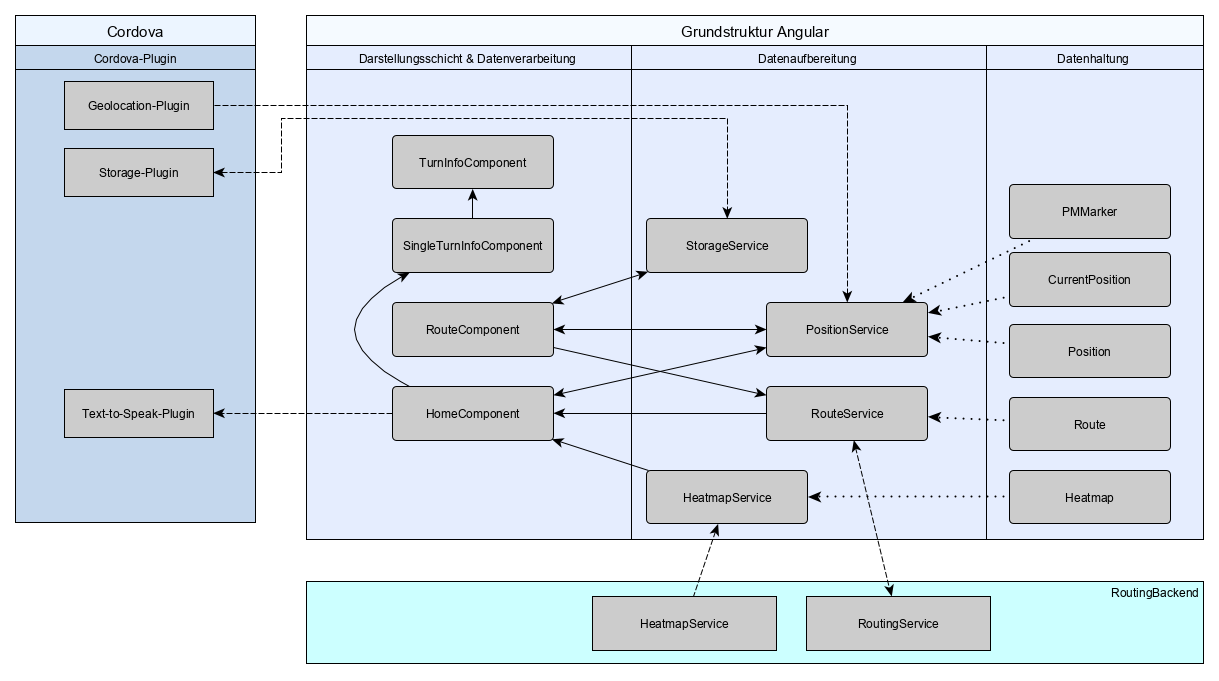
\includegraphics[width=\textwidth]{ressourcen/Architektur-Navigation}
	\caption{Überblick über Navigationsarchitektur}
	\label{fig:ArchtekturNavigation}
\end{figure}

\textbf{Angularbereich}
\\
Die Angular-Applikation besitzt ein zentrales Modul. 
Dieses Modul integriert alle externen Module sowie alle internen Services und Komponenten.
Bei einem Projekt der Größe der Navigationsapplikation ist diese Aufteilung vorteilhaft, da eine bessere Übersicht über alle integrierten Objekte verleiht. 
Bei größeren Applikationen mit mehr Funktionalitäten und mehreren verschiedenen Seiten, würde sich eher eine Aufteilung auf mehrere Module empfehlen. 
Am Anfang der Applikation steht die AppComponent, die sowohl den normalen aufgerufenen Inhalt lädt, als auch die Sidebar beinhaltet. 
Sie enthält somit die Logik der Aufrufmöglichkeit der Sidebar. 
In der Sidebar befindet sich die RouteComponent. 
Diese ist für die Erstellung und Einstellungen der abgerufenen Routen zuständig. 
Datenaustausch passiert in dieser Komponente sowohl mit dem PositionService, um beispielsweise die aktuelle Position zu erhalten, sowie mit dem RouteService. 
In der AppComponent wird die HomePage aufgerufen. 
In dieser werden und alle Funktionen und die Karte selbst aufgerufen. 
Darunter fällt beispielsweise Marker setzen oder die spätere Navigation. 
Dafür benötigt auch sie die Funktionen der RouteService und PositionService, zudem auch noch die Verbindung zum HeatmapService. 
Beim Start der Navigation wird die SingleTurnInfoComponent geladen. 
Diese ist für die grundlegenden Informationen der Route gedacht und bekommt ihre Daten über das Databinding von der HomePage. 
So benötigt sie keine direkte Verbindung zu den Services, da die Daten bereits in der HomePage bereitliegen. 
Bei jeder Veränderung der Daten in HomePage wird dies auch durch das Databinding in die SingleTurnInfoComponent weitergegeben. 
Die letzte Komponente, die TurnsInfoComponent, wird als Modal eingebunden, also eine Oberfläche die im Vordergrund der Applikation zu sehen ist, ohne die anderen Komponenten zu zerstören oder zu verändern. 
Sie bekommt die benötigten Daten von der SingleTurnInfoComponent übergeben und zeigt die Liste aller Richtungsanweisungen an. 


Wie zu Beginn des Kapitels bereits erwähnt, haben die Services die Aufgabe mit den externen Diensten, wie dem Backend des RoutingServices, zu kommunizieren. 
Der PositionService holt sich die aktuelle Position des Mobildevices über eine Erweiterung von Cordova namens Geolocation, die auf native Funktionen dieses Devices zugreift. 
Der RouteService ruft Daten vom Backends ab. 
Dabei werden die Schnittstellen des RoutingServices, die Daten über die möglichen Routen mit speziellen Anforderungen bereitstellen. 
Der HeatmapService kommuniziert mit der Schnittstelle des RoutingBackends, unter der Datenpunkte für eine Heatmap abgefragt werden können. 


\textbf{Cordova}

Das Ionic-Framework nutzt Cordova, um die Angular-Applikation auf einer anderen Plattform auszuführen und einige Vorteile des Devices ausnutzen zu können. 
Das Projekt RiO konzentriert und optimiert dies für Android. 
Die anderen Plattformen werden nicht betrachtet. 
Cordova führt dabei die Angular-Applikation in einem Container aus. 
Das Interface der Appliktion wird dabei über die plattforminterne Webview abgebildet. 
Einer der genutzten Funktionalitäten ist die Positions- und Geschwindigkeitsbestimmung des Gerätes. 
Diese werden über das von Cordova bereitgestellte Geolocationplugin abgerufen. 
Ein weiteres genutztes Plugin ist die Storagefunktion. 
Dies erstellt eine SQLite auf dem Device in die wir Daten speichern können. 
Die letzte Funktion ist Sprachwiedergabe, des Text-to-Speak-Plugins.

\subsection{UIS}
Das folgende Kapitel beschreibt den Aufbau des UIS-Frontends. 
Dieses soll eine Oberfläche für Projektinteressierte sowie für Nutzer des Umweltinformationssystems bieten, indem zum Beispiel die Abdeckung der Sensorknoten in Oldenburg auf einer Karte einsehbar ist sowie eine Exportfunktion der Daten bereitgestellt wird. 


Abbildung \ref{fig:UISArchitekturOverview} zeigt den grundlegenden Aufbau beziehungsweise die zentralen Bausteine des UIS-Fontends.
Das UIS-Frontend selber basiert auf dem Framework-Angular und unterteilt sich somit in Models, Services und Komponenten. Im Fokus stehen für den Aufbau der grundlegenden Webseite die Komponenten. 


\begin{figure}[!htb]
	\centering
	\includegraphics[width=\textwidth]{ressourcen/generiert/Architektur_UIS_Overview}
	\caption{Überblick über die Bestandteile der UIS-Architektur}
	\label{fig:UISArchitekturOverview}
\end{figure}


 
Grundsätzlich kann auf die Seiten „Mitmachen“, „Über uns“ und  „Maps“ zugegriffen werden. Diese sind wiederum in die Kopfzeile beziehungsweise „Navbar“ eingebettet. 
Über die Fußzeile kann zudem auf das Impressum sowie auf die Datenschutzhinweise zugegriffen werden. 
Die wohl wichtigste Komponente des UIS-Frontends ist die Maps-Component in welche zudem die Controller-Component und die Sidebar-Component eingebettet sind. 
Diese greifen auf die unterschiedlichen Services zurück, um zum Beispiel die Sensorknoten auf einer Karte mit den entsprechenden Informationen (wie Koordinaten, Name, ID usw.) abzufragen und anzuzeigen. 
Wie ein Ablauf der Anfrage an die IoT-Plattform aussieht ist in Abbildung \ref{fig:UISArchitekturSequence} dargestellt. 

\begin{figure}[!htb]
	\centering
	\includegraphics[width=\textwidth]{ressourcen/generiert/Architektur_UIS_Sequence}
	\caption{Beispielhafter Ablauf bei Abfrage von Daten der IoT-Plattform über einen Service des UIS-Frontends}
	\label{fig:UISArchitekturSequence}
\end{figure}

Dieser beginnt damit, dass ein User die Maps-Component aufruft, indem er die Seite in der Navbar anklickt.
Daraufhin wird die Seite neu geladen und in welcher die Map initialisiert wird. 
Darauf folgt die getSensornodes-Abfrage an die IoT-Plattform mit welcher die Sensorknoten und die jeweilige Informationen zu diesen abgefragt werden. 
Bevor die Abfrage gestellt werden kann, muss diese über ein Token autorisiert werden.
Die abgefragten Daten werden dann über die einzelnen Komponenten zurückgegeben, bis sie schließlich in der Karte für den Enduser sichtbar werden.
Zudem können über die Chart-Component in Verbindung mit dem ChartService die erhobenen Daten des Sensorknotens in einer Zeitreihe angezeigt werden. 

Um die Übersicht der Sensorknoten in Oldenburg zu verbessern und die Belastung durch Feinstaub bewerten zu können, wird in der Maps-Component auf den HeatmapService zugegriffen. 
Dieser erzeugt in einem vorher bestimmten Kartenausschnitt eine Heatmap auf Basis der Feinstaubwerte, sodass ein Überblick über die Belastung entsteht.
Grundsätzlich greifen alle Services im UIS-Frontend auf die Daten der IoT-Plattform zu den Sensorknoten zu. 
Vom Frontend selber werden keine Schnittstellen zu anderen Teilprojekten der Projektgruppe bereitgesetllt.


Neben den Services und Components existieren mehrere Models um Daten abzuspeichern. 
Diese werden unter anderem zum Speichern der Sensordaten genutzt, sodass hier festgelegt werden kann, welche Daten zu einem Sensorknoten gespeichert werden, um diese anschließend zum Beispiel in der Sidebar-Component anzeigen zu können. 
Ein solches Model wird im UIS-Frontend für die Heatmap, die Sensorknoten, die Zeitreihen und für die Markierungen auf der Karte genutzt.


Zusammenfassend kann zur Architektur oder eher Beschreibung des UIS-Frontends gesagt werden, dass diese durch die Verwendung des Angular-Frameworks jederzeit ausgeweitet werden kann. Es wurde daher keine gesonderte Architektur für das Frontend geplant, sondern die Webseite je nach Bedarf um Komponenten, Services und Models erweitert, um die vorher gestellten Anforderungen zu erfüllen. Hinzu kommt der Zeitdruck während der Projektphase, der eine umfassende Planung des UIS-Frontends nicht ermöglicht hat. Eine solche Planung wird jedoch von der Projektgruppe nicht als notwendig angesehen, da die Grundlagen durch die Anwendung von Angular schon vorhanden sind. 

\subsection{SV Frontend}
Im folgenden Kapitel wird der Aufbau des SV-Frontends beschrieben. Das Ziel des SV-Frontends ist es, den PG RiO Entwicklern die Möglichkeit zu bieten, Sensorknoten zu verwalten. Dazu gehört beispielsweise eine Übersicht aller Sensorknoten, die Daten zur IoT-Plattform senden oder, dass die Informationen dieser Sensorknoten verändert werden können. In Abbildung \ref{fig:SVArchitecture} ist der grundlegende Aufbau, also die zentralen Kompoenten, des SV-Frontends dargestellt. \newline
Da auch dieses Frontend auf dem Framework Angular basiert, ist die Architektur bereits festgelegt und gliedert sich also in Models, Services und Komponenten. Daher wird im folgenden lediglich auf die einzelnen Komponenten und deren Aufgabe eingegangen. Grundsätzlich gibt es folgende Seiten:
\begin{itemize}
	\item  \textit{Sensorknotenübersicht}
	\item \textit{Sensorknoten verändern}
	\item \textit{Config verändern} 
	\item \textit{Sensorknoten hinzufügen}
\end{itemize}
Diese Komponenten sind in der \textit{Navbar}, also der Kopfzeile, eingebettet. \newline
Die Sensornode-Overview-Component hat das Ziel alle Sensorknoten tabellarisch anzuzeigen, die in der Datenbank hinterlegt sind. Um die Sensorknoten und deren Informationen anzeigen zu lassen fragt der Service GetAllSensornodeData diese Informationen an der IoT-Plattform ab. Die Component greift auf diesen Service zu, um so die abgefragten Informationen anzeigen zu können. \newline
Die Component Sensornode-Update hat ebenfalls die Aufgabe alle verfügbaren Sensorknoten tabellarisch anzuzeigen. Jedoch dürfen in dieser Tabelle einige Informationen der Sensorknoten verändert werden. Das kann beispielsweise der Name des Sensorknotens sein oder die Geoposition. Zusätzlich zu dem Service GetAllSensornodeData, greift die Component auf den Service Sensornode-Update zu. Sobald eine Veränderung eines Sensorknotens gespeichert wurde schickt die Component die veränderten Datan an den Sensornode-Update Service. Dieser stellt eine Anfrage bei der Iot-Plattform, das die Daten des Sensorknotens in der Datenbank verändert werden. \newline
Die Veränderung der Konfiguration von virtuellen Sensorknoten wird von der Sensornode-Config-Component übernommen. Diese Component greift ebenfalls auf den GetAllSensornodeData Service zu, um die aktuellen Informationen der Sensorknoten anzeigen zu lassen. Außerdem greift die Component auf den Service Sensornode-Config zu, um die veränderte Konfiguration an die IoT-Plattform zu senden. Aktuell ist es nur möglich die Konfiguration von virtuellen Sensorknoten zu verändern. Jedoch kann diese Component so erweitert werden, dass ebenfalls die Konfiguration von physischen Sensorknotenverändert werden kann. Die Veränderung der Konifguration von virtuellen Sensorknoten kann das Messintervall und die Mock Werte der Umweltdaten bewirken. \newline 
Und letztendlich hat die Sensornode-New-Component die Aufgabe, neue Sensorknoten dem System hinzuzufügen. Es können entweder virtuelle oder physische Sensorknoten dem System hinzugefügt werden. Dazu gehört zum einen das Hinterlegen der Informationen des Sensorknotens zur Datenbank und zum anderen das Hinterlegen der Zugangsdaten, damit der Sensorknoten sich mit dem MQTT Broker verbinden kann. Um die Daten an die IoT-Plattform zu senden greift die Component auf den Service Sensornode-New zu. Beim Neuanlegen eines Sensorknotens ist zu beachten, dass die hinzugefügten Sensorknoten lediglich in der Datenbank hinterlegt werden. Das bedeutet, dass die neu angelegten Sensroknoten sofort Daten senden und diese im UIS-Frontend einsehbar sind. Insbesondere wenn ein virtueller Sensorknoten angelegt wird, muss dieser zunächst deployed werden. \newline
Neben den Components und Services existieren Models zur Speicherung von Daten. Aktuell gibt es lediglich ein Model, das zur Speicherung der Sensorknoten dient. Das Model legt fest, welche Daten zu einem Sensorknoten gespeichert werden, um diese zum Beispiel in der Sensorknotenübersicht dazustellen. Jedoch können beliebig viele Models nach Bedarf hinzugefügt werden. \newline
Zusammenfassend kann zur Architektur dieses Frontends gesagt werden, dass diese erweiterbar ist. Durch die Verwendung von Angular können sehr einfach neue Components hinzugefügt werden, die eine neue Seite auf der Oberfläche darstellen. Außerdem können einige Components und deren Services erweitert werden, wie zum Beispiel die Component Sensornode-Config. Diese kann so erweitert werden, dass auch die Konfiguration von physischen Sensorknoten verändert werden kann. Außerdem wäre es bei der Component Sensornode-Update wünschenswert gewesen, neben dem Verändern von Sensorknotendaten, auch die Möglichkeit zu haben, Sensorknoten aus dem System zu entfernen. Diese Anpassungen waren zeitlich nicht umsetzbar, jedoch sind die beiden zuvor genannten Szeanrien auf der Datenbank ausführbar. Somit wurden diese Anforderungen nicht als zwingend notwendig angesehen werden. 

\begin{figure}[!htb]
	\centering
	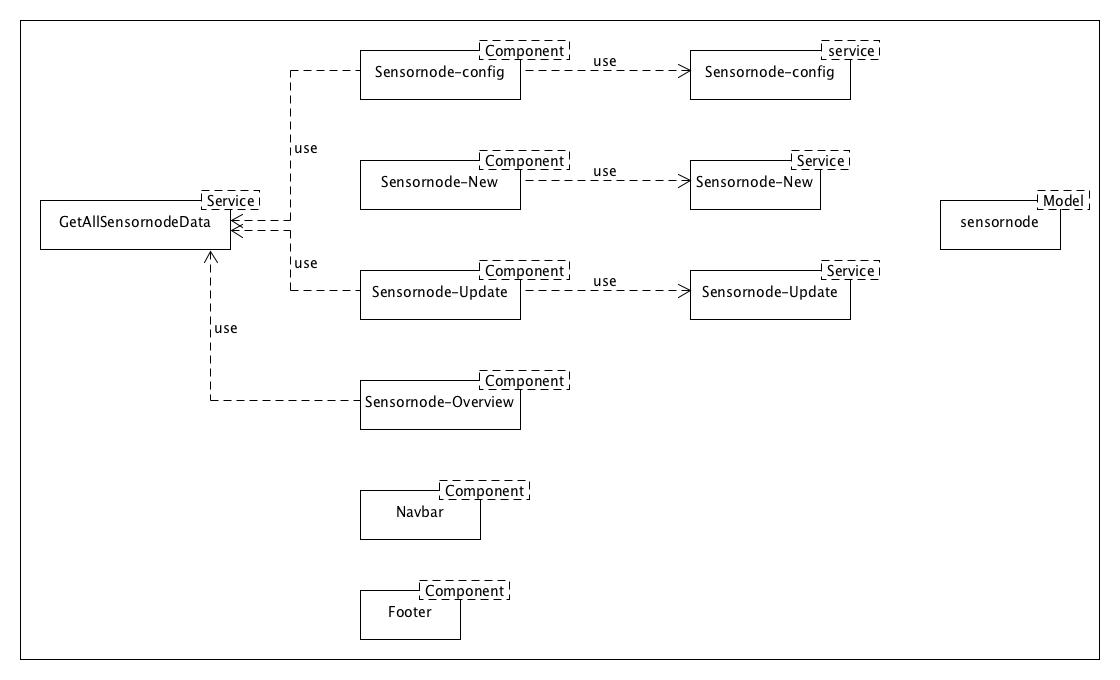
\includegraphics[width=\textwidth]{ressourcen/svArchitecture.jpg}
	\caption{Überblick über die Bestandteile der SV-Architektur}
	\label{fig:SVArchitecture}
\end{figure}
